\documentclass[11pt,answers]{exam}

\usepackage{etex}
\usepackage{amssymb,amsmath,multicol} %<-- InWorksheetExam1 i also have fancyhdr,

\usepackage[metapost]{mfpic}
\usepackage[pdftex]{graphicx}
\usepackage{tabu}

\usepackage{pst-plot}
\usepackage{pgfplots}
\pgfplotsset{compat=1.9}

\usepackage{tikz}
\usepackage{tkz-2d}
\usepackage{tkz-base}
\usetikzlibrary{calc}
\usetikzlibrary{arrows}

\usepackage{systeme}

\usepackage[inline]{enumitem}
\usepackage{refcount}%<-- non in WorksheetExam1

\usepackage{pstricks-add,pst-eucl}
\usepackage{systeme}
\usepackage{setspace}
\usepackage{multicol}


\usepackage[inline]{enumitem}   
\makeatletter
% This command ignores the optional argument for itemize and enumerate lists
\newcommand{\inlineitem}[1][]{%
\ifnum\enit@type=\tw@
    {\descriptionlabel{#1}}
  \hspace{\labelsep}%
\else
  \ifnum\enit@type=\z@
       \refstepcounter{\@listctr}\fi
    \quad\@itemlabel\hspace{\labelsep}%
\fi}
\makeatother


\def\f{x+1} \def\g{-x/3+2}  \def\h{-x+3}

\newcommand{\vasymptote}[2][]{
    \draw [densely dashed,#1] ({rel axis cs:0,0} -| {axis cs:#2,0}) -- ({rel axis cs:0,1} -| {axis cs:#2,0});
}

\boxedpoints

\addpoints
%\printanswers
\noprintanswers

\opengraphsfile{Q11a_Fa18}

\begin{document}
\extrawidth{-0.3in}
\pagestyle{headandfoot}

\setlength{\hoffset}{-.25in}

\extraheadheight{-.3in}
\runningheadrule
\firstpageheader{\bfseries {Precalculus}}{ \bfseries {Quiz 11 }}{\bfseries {12/4/18}} 

\begin{center}
	This quiz has \numquestions\ questions, for a total of \numpoints\
	points and \numbonuspoints\ bonus points.
\end{center}


\firstpagefooter{} %%&&CHANGED
                {}
                {%Points earned: \hbox to 0.5in{\hrulefill}
                % out of  \pointsonpage{\thepage} points
                }
                 
						

\vspace*{0.1cm}
\hbox to \textwidth { \scshape {Name:} \enspace\hrulefill}
\vspace{0.1cm}




\pointpoints{point}{points}

\begin{questions}


\addpoints


 \question Part of the graph of a sinusoidal function  is shown below:
 
\begin{mfpic}[25]{-2}{8}{-6}{2}
\point[3pt]{(1,1), (2.5,-2),(4,-5), (5.5,-2), (7, 1)}
\tlabel(0.75,1.25){\tiny $\left(1,1\right)$}
\tlabel[cc](2,-2.25){\tiny $\left(2.5,-2\right)$}
\tlabel(3.75,-5.35){\tiny $\left(4,-5\right)$}
\tlabel[cc](6,-2.25){\tiny $\left(5.5,-2\right)$}
\tlabel(6.75,1.25){\tiny $\left(7,1\right)$}
\axes
\tlabel[cc](8,-0.25){\scriptsize $x$}
\tlabel[cc](0.25,2){\scriptsize $y$}
%%\tcaption{Extending the graph of $y = f(x)$.}
\xmarks{-1,1,2,3,4,5,6,7}
\ymarks{-6,-5,-4,-3,-2,-1,1}
\tlpointsep{4pt}
\axislabels {x}{{\tiny $-1 \hspace{7pt}$} -1, {\tiny $1$} 1,  {\tiny $2$} 2,  {\tiny $3$} 3,  {\tiny $4$} 4,  {\tiny $5$} 5,  {\tiny $6$} 6,  {\tiny $7$} 7}
\axislabels {y}{{\tiny $-5$} -5, {\tiny $-4$} -4,{\tiny $-3$} -3,{\tiny $-2$} -2,{\tiny $-1$} -1, {\tiny $1$} 1}
\dotted \function{-1, 1, 0.1}{3*cos(3.14159265*(x-1)/3)-2}
\function{1, 7, 0.1}{3*cos(3.14159265*(x-1)/3)-2}
\end{mfpic}
 
 \begin{parts}
 	\part[1] The amplitude is: \hbox to 1in{\dotfill} 
 	\part[1] The period is: \hbox to 1in{\dotfill}
 	\bonuspart[1] The equation of the midline is: \hbox to 1in{\dotfill}
 	\part[2]  Write  an equation that represents the curve in the form
 	 $\displaystyle y = a \cos B(x - h)+k$. Show evidence of Your thinking, and write your equation in the space provided below.
 	
 	
 	\fillwithdottedlines{0.8in}
 	\medskip
 	
 	The equation is $y=$\dotfill
 	
 \end{parts}
 
 \question  As a wave passes by an offshore piling, the height of the water is modeled by the function
$\displaystyle  h(t) = 7 \cos \left ( \frac{\pi}{20}t\right )$,  where $h(t)$ is the height in feet above mean sea level at time $t$ seconds.
\begin{parts}
	\part[2] Find the period of the wave. Show evidence of Your thinking.
	\fillwithdottedlines{0.8in}
	\part[2] Find the wave height, that is, the vertical distance between the trough and the crest of the wave. Show evidence of Your thinking.
	\fillwithdottedlines{0.8in}
	\end{parts}
\end{questions}
\newpage

\par\medskip\hrule\medskip


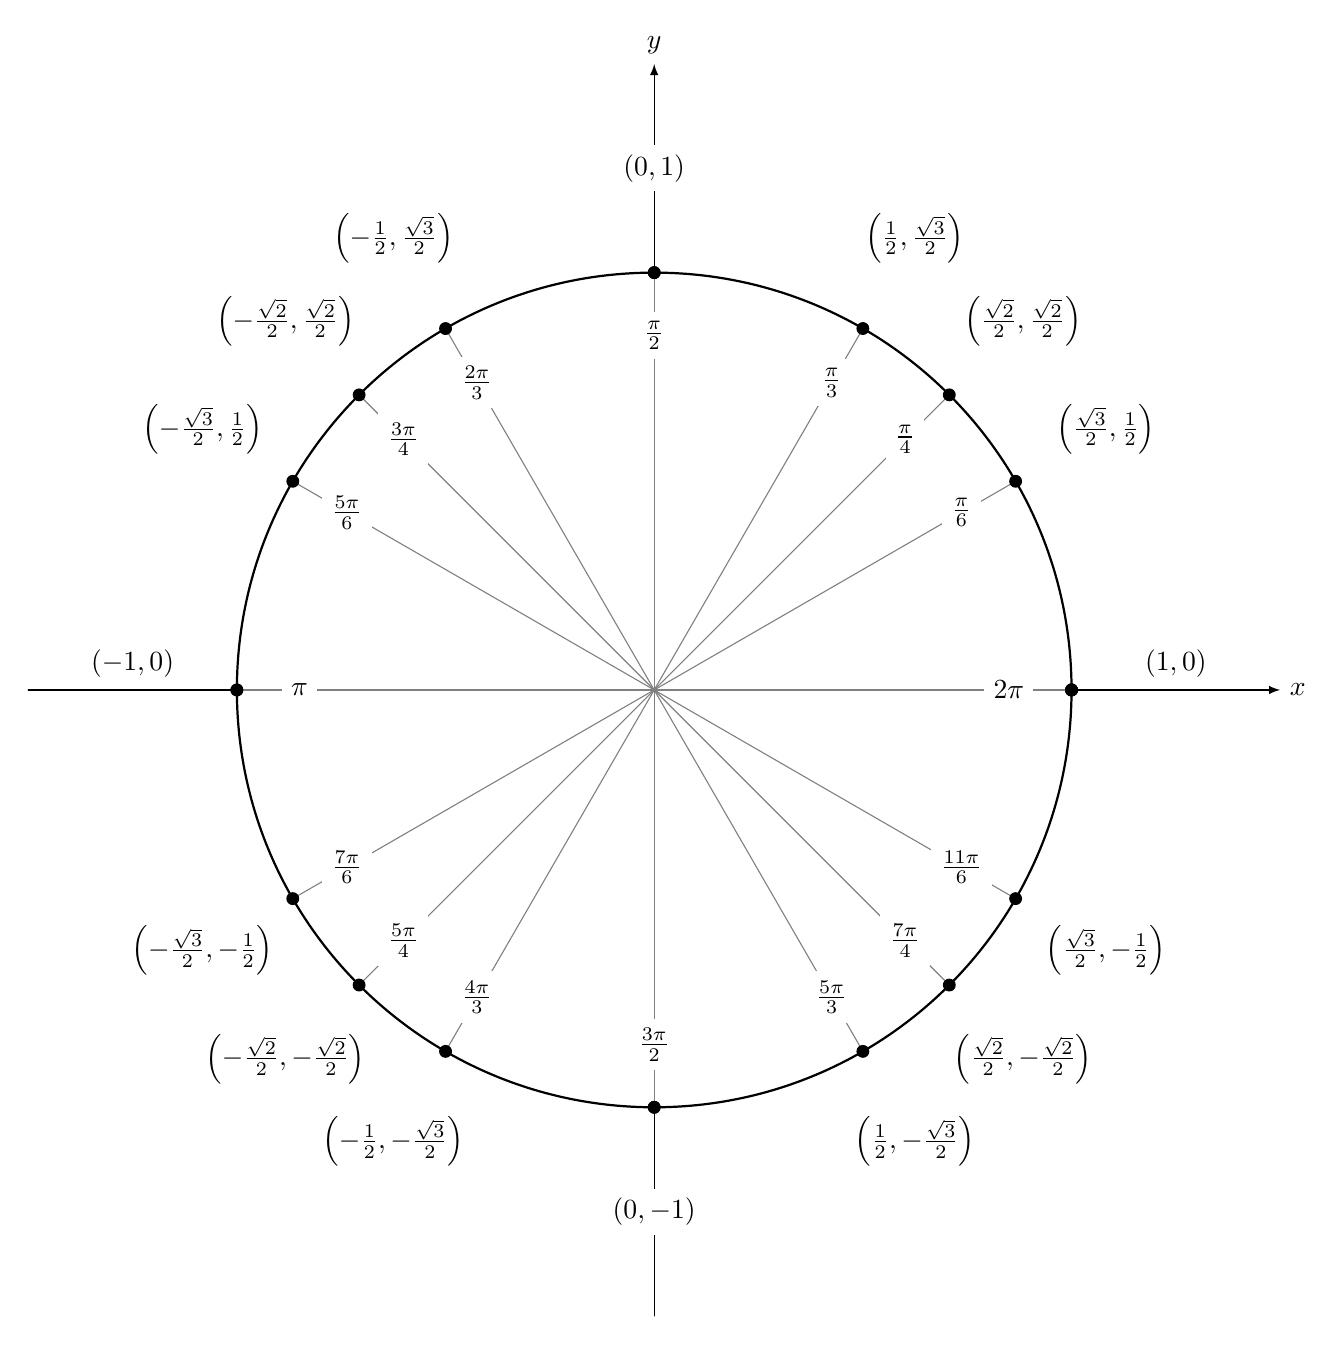
\begin{tikzpicture}[scale=5.3,cap=round,>=latex]
% draw the coordinates
\draw[->] (-1.5cm,0cm) -- (1.5cm,0cm) node[right,fill=white] {$x$};
\draw[->] (0cm,-1.5cm) -- (0cm,1.5cm) node[above,fill=white] {$y$};

% draw the unit circle
\draw[thick] (0cm,0cm) circle(1cm);

\foreach \x in {0,30,...,360} {
	% lines from center to point
	\draw[gray] (0cm,0cm) -- (\x:1cm);
	% dots at each point
	\filldraw[black] (\x:1cm) circle(0.4pt);
	% draw each angle in degrees
	%\draw (\x:0.6cm) node[fill=white] {$\x^\circ$};
}

\foreach \x in {0,45,...,360} {
	% lines from center to point
	\draw[gray] (0cm,0cm) -- (\x:1cm);
	% dots at each point
	\filldraw[black] (\x:1cm) circle(0.4pt);
	% draw each angle in degrees
	%\draw (\x:0.6cm) node[fill=white] {$\x^\circ$};
}
% draw each angle in radians
\foreach \x/\xtext in {
	30/\frac{\pi}{6},
	45/\frac{\pi}{4},
	60/\frac{\pi}{3},
	90/\frac{\pi}{2},
	120/\frac{2\pi}{3},
	135/\frac{3\pi}{4},
	150/\frac{5\pi}{6},
	180/\pi,
	210/\frac{7\pi}{6},
	225/\frac{5\pi}{4},
	240/\frac{4\pi}{3},
	270/\frac{3\pi}{2},
	300/\frac{5\pi}{3},
	315/\frac{7\pi}{4},
	330/\frac{11\pi}{6},
	360/2\pi}
\draw (\x:0.85cm) node[fill=white] {$\xtext$};

\foreach \x/\xtext/\y in {
	% the coordinates for the first quadrant
	30/\frac{\sqrt{3}}{2}/\frac{1}{2},
	45/\frac{\sqrt{2}}{2}/\frac{\sqrt{2}}{2},
	60/\frac{1}{2}/\frac{\sqrt{3}}{2},
	% the coordinates for the second quadrant
	150/-\frac{\sqrt{3}}{2}/\frac{1}{2},
	135/-\frac{\sqrt{2}}{2}/\frac{\sqrt{2}}{2},
	120/-\frac{1}{2}/\frac{\sqrt{3}}{2},
	% the coordinates for the third quadrant
	210/-\frac{\sqrt{3}}{2}/-\frac{1}{2},
	225/-\frac{\sqrt{2}}{2}/-\frac{\sqrt{2}}{2},
	240/-\frac{1}{2}/-\frac{\sqrt{3}}{2},
	% the coordinates for the fourth quadrant
	330/\frac{\sqrt{3}}{2}/-\frac{1}{2},
	315/\frac{\sqrt{2}}{2}/-\frac{\sqrt{2}}{2},
	300/\frac{1}{2}/-\frac{\sqrt{3}}{2}}
\draw (\x:1.25cm) node[fill=white] {$\left(\xtext,\y\right)$};

% draw the horizontal and vertical coordinates
% the placement is better this way
\draw (-1.25cm,0cm) node[above=1pt] {$(-1,0)$}
(1.25cm,0cm)  node[above=1pt] {$(1,0)$}
(0cm,-1.25cm) node[fill=white] {$(0,-1)$}
(0cm,1.25cm)  node[fill=white] {$(0,1)$};
\end{tikzpicture}



\end{document}                 